\chapter{Ansätze und Related Work}
\label{cha:Ansaetze}
Wir haben \textit{Trajektorienplanung}, \textit{\acrlong{RL}} und \textit{Spieltheorie} als vielversprechendste Ansätze für Spe\_ed erachtet und genauer unter die Lupe genommen. Die folgenden Unterkapitel fassen unsere Erkenntnisse zur Anwendbarkeit der jeweiligen Ansätze und Untersuchungen verwandter Arbeiten zusammen.

\section{Trajektorienplanung}

Spe\_ed kann wie folgt betrachtet werden: F\"ur einen Agenten m\"ussen Steuerbefehle erzeugt werden, die zu einer Reihe von Wegpunkten mit Geschwindigkeiten - also einer Trajektorie - f\"uhren. Der Pfad soll zudem Kollisionen vermeiden. Diese Betrachtungsweise f\"uhrt zum Ansatz, das Problem mithilfe von Trajektiorienplanung aus der klassischen Robotik zu l\"osen. Einige der prominentesten Vertreter dieser Algorithmen sind \acrfull{VFH} \cite{Borenstein.}, \acrfull{RRT}\cite{S.Karaman.2011}, Voronoi-Diagramm \cite{Garrido.2006}, und \acrfull{APF} \cite{Raja.2012}. Wir haben uns entschieden, den letztgenannten Ansatz zu testen, da dieser die Umgebung in einer f\"ur Spe\_ed passend erscheinenden Weise darstellt. Beim \acrshort{APF} wird die Umgebung als ein Feld von Potenzialen modelliert, bspw. indem Hindernisse ein hohes abstoßendes Potenzial erhalten. Der Agent bestimmt dann zur Pfadplanung den Weg des steilsten Abstiegs (\"uber den Gradient). Passend f\"ur Spe\_ed, da große Freifl\"achen bevorzugt und Gegner gemieden werden. Zudem kann der Algorithmus mit evolution\"aren Ans\"atzen kombiniert werden, woraus bspw. das \acrfull{EAPF} entsteht. \cite{Raja.2012} 

Der L\"osungsansatz alleine \"uber Trajektorienplanung bringt allerdings einige Probleme mit sich. Das Bedeutendste ist, dass Trajektorienplanung alleine keine Strategie finden kann. Vielmehr implementiert es eine zuf\"allige oder vom Entwickler erdachte Strategie, z.B. \glqq halte m\"oglichst großen Abstand zu Hindernissen\grqq. Das ist auch dadurch bedingt, dass in der klassischen Robotik meist ein Ziel wie \glqq fahre diesen Punkt an\grqq{} oder \glqq halte genau diesen Abstand zum Fahrer vor dir\grqq{} vorgegeben ist. In unserer Aufgabe ist das Ziel zu abstrakt (\glqq gewinne das Spiel\grqq{}/\glqq Überlebe länger als die anderen\grqq{}). Besonders das evaluierte \acrshort{APF} schafft es mit der typischen Parameterkonfiguration nicht Gegner abzuschneiden oder den Platz nahe an W\"anden effizient zu nutzen.\footnote{W\"ande erhalten normalerweise ein abstoßendens Potenzial, allerdings ist es an sich sinnvoll, nahe heranzufahren.} Aus den genannten Gr\"unden wurde dieser als alleiniger wieder verworfen, allerdings taucht das Voronoi-Diagramm im finalen Ansatz auf.

\section{\acrlong{RL}}
% kurze Einleitung
In den letzten Jahren haben \acrshort{RL}-Algorithmen beeindruckende Fortschritte gezeigt. Mittlerweile übertreffen sie beispielsweise menschliche Spitzenleistungen in Atari-Spielen, Schach, Shogi, Go und Dota 2 \cite{Mnih.19.12.2013, Silver.2018b, OpenAI.2019}. Daher ist es nur naheliegend, \acrshort{RL} auch für den diesjährigen InformatiCup als Ansatz in Betracht zu ziehen.

% Kurze RL-Def
\acrshort{RL} beschäftigt sich mit der Fragestellung, wie Software-\textit{Agenten} lernen können, eine bestimmte Aufgabe in einer bestimmten \textit{Umgebung} zu meistern \cite{Sutton.1998}. Im Bezug auf den diesjährigen InformatiCup ist die Umgebung das Spiel Spe\_ed, der Agent ein Spieler und die Aufgabe zu gewinnen. Es gibt allerdings noch ein paar Eigenheiten von Spe\_ed, die die Anwendung von \acrshort{RL} erschweren: (1) Die Spielfeldgröße ist variabel, (2) Die Anzahl der Gegenspieler ist variabel, (3) Die \textit{Policy} (Verhaltensweise) der Gegenspieler ist unbekannt.

% MDP
Der Lernprozess bei \acrshort{RL} wird typischerweise durch den \acrfull{MDP} beschrieben: Der Agent führt in jedem Zeitschritt $t$ eine Aktion $a_t$ aus, die den Zustand $s_t$ der Umgebung verändert. Nachdem $a_t$ ausgeführt wurde, empfängt der Agent von der Umgebung einen neuen Zustand $s_{t+1}$ und eine Belohnung $r_{t+1}$. Die \textit{Policy} $\pi$ eines Agenten legt die Aktion fest, die er in einem bestimmten Zustand ausführt. Genauer ist $\pi(a|s)$ die Wahrscheinlichkeit, dass der Agent die Aktion $a$ im Zustand $s$ wählt. Ziel eines \acrshort{RL}-Algorithmus ist, eine Policy zu erlernen, die die akkumulierten, in Zukunft erwarteten Belohnungen - kurz: \textit{Return} - maximiert. \cite{Sutton.1998}

% Zustandsraum
Um \acrshort{RL} auf Spe\_ed anzuwenden, müssen wir also erst einmal den Zustandsraum modellieren. Dabei kommen einem bereits die Variabilität der Spielfeldgröße und der Spieleranzahl in die Quere. Denn an sich könnte man einen Spielzustand vollständig beschreiben, wenn man den Zustandsraum mit folgenden Informationen ausstattet:
\begin{itemize}
	\item Die Belegung der Felder auf dem Spielfeld (mit möglichen Zahlencodierungen -1 bis \# Spieler)
	\item Die Positionen aktiver Spieler
	\item Die Bewegungsrichtungen aktiver Spieler
	\item Die Geschwindigkeiten aktiver Spieler
	\item Einen Rundenzähler
\end{itemize}
\acrshort{RL}-Algorithmen fordern allerdings eine Zustandsdarstellung mit einer festen Anzahl an Zustandsattributen. Zur Lösung dieses Problems gibt es zwei Ansätze: (1) Die maximal mögliche Zustandsgröße wählen und kleinere Zustände mit bestimmten \textit{Padding-Werten} auf die maximale Größe erweitern. (2) Nur einen Ausschnitt der Umgebung mit fester Größe betrachten (z.B. nur x Felder in jede Richtung um den Agenten herum und nur die nächsten y anderen Spieler betrachten). Dabei können beide Ansätze miteinander kombiniert werden. In jedem Fall steht jedoch fest, dass der Zustandsraum sehr groß ist - ein Spielfeld der Größe 50x50 mit 5 Spielern hätte mit den oben aufgelisteten Informationen modelliert \[Höhe*Breite+4*Spieler+1=50*50+4*5+1=2.521\] Zustandsattribute. Um den Ansatz nicht von vorn herein zu verkomplizieren, haben wir zunächst eine kleine, feste Spielfeldgröße und nur einen Gegenspieler als Umgebung angenommen.

% Self-Play
Bevor wir uns nun mit den eigentlichen \acrshort{RL}-Algorithmen beschäftigen können, muss allerdings noch eine weitere Frage geklärt werden: Gegen wen spielt unser Agent eigentlich während des Trainings? Man kann den Agent zwar auf einem leeren Spielfeld trainieren, allerdings würde dieser wohl lediglich lernen, alle Felder so langsam wie möglich auszufüllen, um die unausweichliche Eliminierung so lange wie möglich hinauszuzögern.\footnote{Der Agent erhält die Belohnung 1 für einen Siegeszug, -1 bei Eliminierung und sonst 0.} Es kommt auch nicht infrage den Agent gegen einen eigens entwickelten Gegenspieler spielen zu lassen, denn unser Agent würde nur lernen, gegen diesen einen Gegner zu gewinnen. Der derzeit beste Ansatz für solch ein Problem ist das sogenannte \textit{Self-Play}, wie es beispielsweise \textit{Google} und \textit{DeepMind} bei \textit{AlphaZero} \cite{Silver.2018b} und \textit{OpenAI Five} \cite{OpenAI.2019} verwenden. Hierbei tritt der Agent immer wieder gegen sich selbst an und lernt somit automatisch gegen Gegenspieler mit unterschiedlicher Policy zu spielen. Um \acrshort{RL}-Agenten letztendlich in Spe\_ed trainieren zu können, haben wir unser Spe\_ed-Modell in ein \textit{Gym-Environment} \cite{Brockman.2016} eingekapselt und die Schnittstellen vektorisiert, um Self-Play zu ermöglichen.

% Q-Learning
Der wohl bekannteste \acrshort{RL}-Ansatz ist das 1989 von Chris Watkins vorgestellte \textit{Q-Learning} \cite{Watkins.1992}. Q-Learning lernt die optimale \textit{Aktionswert-Funktion $q_*$} mit Q zu approximieren. Q wird dabei tabellarisch dargestellt, weshalb der Ansatz nur auf Umgebungen mit diskreter Zustands- und Aktionsdarstellung anwendbar ist. Das ist vorerst kein Problem, da beides bei Spe\_ed diskret dargestellt werden kann. Was hingegen problematisch ist, ist die Größe des Zustandsraumes. Bereits auf einem 3x3 Spielfeld mit 2 Spielern gibt es $4^{3*3}=262.144$ mögliche Belegungen des Spielfelds.\footnote{Die Basis der Berechnung ergibt sich durch $\# Spieler + 2$, da dies der Anzahl der möglichen Belegungen eines Feldes entspricht: -1 (Kollision), 0 (Frei), x (Spieler x)} Das bedeutet, dass alleine durch ein 3x3 Spielfeld - von Informationen über Spielerpositionen etc. abgesehen - eine Q-Tabelle mit $262.144$ Einträgen benötigt wird. Man kann die Q-Tabelle zwar dynamisch gestalten und den Zustandsraum durch Symmetrieüberlegungen etwas verkleinern, allerdings explodiert der Zustandsraum trotzdem spätestens bei Spielfeldern größer als 5x5 zu nicht umsetzbaren Größen. Wir konnten Q-Learning-Agenten zwar erfolgreich auf einem 3x3 Spielfeld trainieren, allerdings können solch kleine Spielfelder auch durch Tiefensuche in sehr kurzer Zeit optimal gelöst werden. Daher ist ein tabellarischer Ansatz ungeeignet.

% DRL - DQN
2013 haben Mnih et al. einen neuen Meilenstein im Bereich des \acrshort{RL} gesetzt, indem Sie \acrfullpl{DNN} als Funktionsapproximatoren zur Approximation der Q-Funktion beim Q-Learning verwenden \cite{Mnih.19.12.2013, Mnih.2015}. Das dabei entstandene \acrfull{DQN} haben Minh et al. erfolgreich verwendet, um Atari 2600 Spiele zu spielen. Im Gegensatz zum tabellarischen Q-Learning können \acrshortpl{DQN} kontinuierliche Zustandsdarstellungen als Eingang verwenden. Das reduziert die Größe der Zustandsdarstellung bei Spe\_ed drastisch - ein 3x3 Spielfeld kann nun unabhängig von der Anzahl der möglichen Belegung eines Feldes mit $3*3=9$ Zustandsattributen beschrieben werden. Des Weiteren können \acrshortpl{DQN} Verallgemeinerungen über Spielzustände lernen. Das hat den Vorteil, dass sie nicht jeden konkreten Spielzustand gesehen haben müssen, um ihn bewerten zu können.

% MLP vs CNN
Statt dem standardmäßigen \acrfull{MLP} haben Mnih et al. ein \acrfull{CNN} als Netzwerkarchitektur verwendet, da sich \acrshortpl{CNN} besonders gut für die Verarbeitung von Bildern (bzw. \textit{Spiel-Frames}) eignen. Bei Spe\_ed reicht eine rein bildliche Darstellung des Spielfelds allerdings nicht zur Beschreibung des Zustands aus - es fehlen die Informationen über Spielerpositionen, -geschwindigkeiten und -bewegungsrichtungen. Daher haben wir eine reine \acrshort{MLP}-Architektur und eine Architektur mit getrennten \acrshort{CNN} und \acrshort{MLP}-Eingangslayer, die in tieferen Layern zusammengeführt werden, auf Spe\_ed getestet. Leider haben beide Architekturen jedoch auch nach längerer Trainingszeit keine guten Ergebnisse geliefert.

% Begründung für Entscheidung gegen RL
Zu diesem Zeitpunkt haben wir uns dafür entschieden, den \acrshort{RL}-Ansatz nicht weiter zu verfolgen und uns auf die Tiefensuche zu konzentrieren. Folgende Probleme vermuten wir als Hauptgründe für das Scheitern: (1) Der Zustandsraum ist selbst kontinuierlich betrachtet sehr groß - deutlich größer als beispielsweise beim Schach; (2) aufgrund unserer begrenzten Ressourcen können wir die \acrshort{DQN}-Architektur nicht tief/groß genug wählen und das \acrshort{DQN} nicht lange genug trainieren; (3) Self-Play kann den Trainingsverlauf destabilisieren und benötigt für erfolgreiche Ergebnisse besonders viel Trainingszeit \cite{Bai.22.06.2020}.


\section{Spieltheorie}
\label{cha:spieltheorie}

Nat\"urlich darf bei den Ans\"atzen zur L\"osung eines Spiels auf keinen Fall die Spieltheorie vergessen werden. Laut Wikipedia ist die Spieltheorie \glqq eine mathematische Theorie, in der Entscheidungssituationen modelliert werden, in denen mehrere Beteiligte miteinander interagieren. Sie versucht dabei unter anderem, das rationale Entscheidungsverhalten in sozialen Konfliktsituationen davon abzuleiten\grqq{} \cite{wikipedia_spieltheorie} - klingt sehr passend.

Bei Spe\_ed handelt es sich um ein Konstantsummenspiel (spieltheoretisch \"aquivalent zum Nullsummenspiel) mit perfekter Information. Wir kennen also das gesamte bisherige Spielgeschehen und wenn wir gewinnen, verliert der Gegner. Ein simpler Gedanke, eine Strategie f\"ur ein derartiges Spiel zu entwerfen ist, alle m\"oglichen Verl\"aufe aufzuz\"ahlen und den Gewinner am Ende zu bestimmen. Somit k\"onnten wir in jeder Situation den Zug w\"ahlen, bei dem wir am Ende gewinnen.\footnote{Vorausgesetzt, die Gegner spielen nicht perfekt. Wenn alle Spieler perfekt spielen, gewinnt der mit der besten Startposition.} 

Da Spe\_ed aus spieltheoretischer Sicht damit dem Schach sehr \"ahnlich ist, erwies sich eine Analyse der dort verwendeten Techniken als sinnvoll. Die meisten Algorithmen f\"ur Schach verwenden diese Suchb\"aume bzw. Spielb\"aume in verschiedenen Formen und Kombinationen. F\"ur uns erschien der Minimax-Algorithmus gut anwendbar.

Dabei wird ein Suchbaum aufgebaut, der alternierend Ebenen enth\"ahlt in denen der eigene Spieler bzw. der gegnerische Spieler am Zug ist. Der eigene Spieler versucht seinen Gewinn zu maximieren, daher sind dies die maximierenden Levels. Die Gegner versuchen den Gewinn vom eigenen Spieler zu minimieren, dies sind daher die minimierenden Levels. \cite{Shannon.1950, Campbell.1983}

Versuchen wir einen Suchbaum nun am Beispiel eines 4x4 Feldes mit zwei Spielern aufzustellen. Für den ersten Zug hat jeder Spieler 5 M\"oglichkeiten seine Aktion zu w\"ahlen,\footnote{Praktisch  können es auch weniger sein, in der ersten Runde bspw. f\"uhrt slow\_down zu Geschwindigkeit 0. Hier soll es allerdings um eine Worst-Case Absch\"atzung gehen.} das ergibt $5^{2} = 25$ Spielsituationen nach Runde eins. Nun kann wieder jeder Agent aus 5 Aktionen w\"ahlen, dadurch kommen  $5^{2} = 25$ M\"oglichkeiten zustande, in Runde zwei zu agieren. Insgesamt k\"onnen also auf 25 Situationen 25 M\"oglichkeiten gebaut werden, f\"ur Runde zwei ergeben sich dadurch $(5^{2})^{2} = 625$ Situationen. In Runde drei stehen nun 625 Situationen zur Verf\"ugung, wieder gibt es 25 Kombinationen darauf zu agieren, also $625 \cdot 25 = 15625$. In Runde vier gibt es bereits 390.625 Zust\"ande, in Runde f\"unf 9.765.625, in Runde $n$: $(5^{2})^{n}$. Bei einem Spiel auf 4x4 mit zwei Spielern kann es maximal $16 / 2 - 1 = 7$ Runden geben, daf\"ur gibt es 6.103.515.625 Spielverl\"aufe. Der Zustandsraum ist also (v.a. f\"ur gr\"ossere Felder) zu gewaltig, um alle Verl"aufe aufzuz\"ahlen. Allerdings erweisen sich einige Pfade relativ schnell als unbrauchbar wegen eines zu schlechten Ergebnisses in diesen Pfaden. Um diese Pfade auszuschließen und damit eine Beschleunigung zu erreichen, ist ein vielgenutztes Verfahren das Alpha-Beta-Pruning \cite{Knuth.1975}. Hierzu werden zwei Werte \textit{Alpha} und \textit{Beta} eingeführt, die den minimalen Wert, den der maximierende Spieler bzw. den maximalen Wert, den der minimierende Spieler erreichen kann, darstellen. Sobald in einem Teilbaum klar ist, dass dieser kein besseres Ergebnis (bzw. schlechteres bei gegnerischem Spieler) erreichen kann, wird dieser ausgeschlossen. Dies ist in Abb. \ref{fig:alphabeta} dargestellt.


\begin{figure}[h]
    \centering
    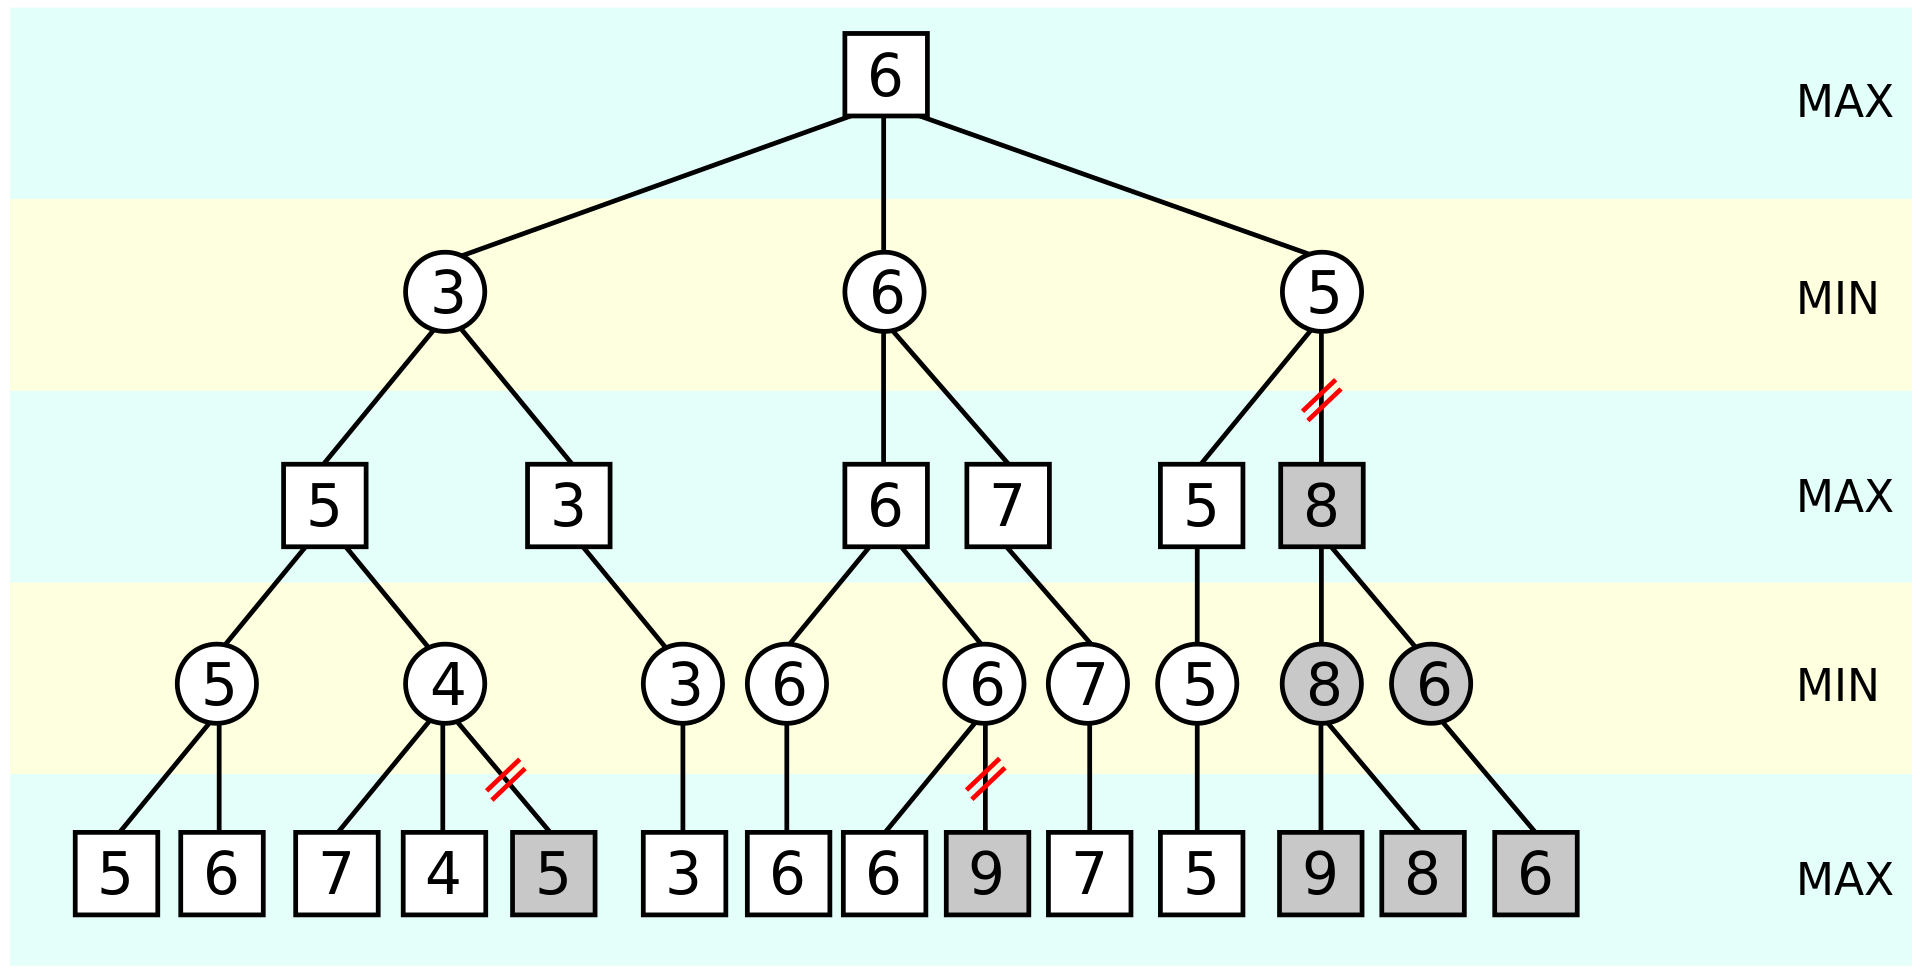
\includegraphics[width=\textwidth]{img/AB_pruning.svg.png}
    \caption[Minimax mit Alpha-Beta-Pruning]{Minimax mit Alpha-Beta-Pruning. Graue Pfade werden nicht beachtet, da sie auf jeden Fall nichts mehr am Ergebnis verbessern. Abbildung aus \cite{wikipedia_alpha_beta} entnommen.}
    \label{fig:alphabeta}
\end{figure}

Trotz der Reduktion der Pfade durch Alpha-Beta-Pruning ist es meist nicht möglich, alle Pfade bis auf die unterste Tiefe zu berechnen. Der Suchbaum kann stattdessen nur bis zu einer gewissen Tiefe durchsucht werden. Allerdings steht der Sieger in dieser Tiefe oftmals noch nicht fest - wie also zwischen den Aktionen w\"ahlen? An dieser Stelle kommt nun die Bewertungsfunktion ins Spiel. So wird bspw. mittels einer Heuristik die Situation bewertet. F\"ur Spe\_ed hat sich Voronoi als eine passende Bewertungsheuristik ergeben.

Die meisten Arbeiten beschäftigen sich mit Zwei-Spieler-Problemen. Bei Spe\_ed handelt es sich jedoch um ein Multi-Player-Problem. Perez und Oommen stellen in \cite{Perez.2019} eine einfache Erweiterung des Minimax-Algorithmus auf mehrere Spieler vor.


